

\documentclass[9pt]{beamer}

\usetheme[numbering=fraction, sectionpage=none,titleformat=smallcaps]{metropolis}


%\useoutertheme{smoothbars}
%\setbeamercolor{mini frame}{fg=white, bg=black}
%\setbeamercolor{section in head/foot}{fg=white, bg=black}

% !TEX TS-program = pdflatex
% !TEX encoding = UTF-8 Unicode


%%%%%%%%%%%%%%%%%%%%%%%%
% Usual LaTeX Packages %
%%%%%%%%%%%%%%%%%%%%%%%%

\usepackage{amsmath}
\usepackage{amsfonts}
\usepackage{amssymb}
\usepackage{graphicx}
\usepackage{mathrsfs} 			% For Weinberg-esque letters
\usepackage{cancel}				% For "SUSY-breaking" symbol
\usepackage{slashed}            % for slashed characters in math mode
\usepackage{bbm}                % for \mathbbm{1} (unit matrix)
\usepackage{amsthm}				% For theorem environment
\usepackage{multirow}			% For multi row cells in table
\usepackage{arydshln} 			% For dashed lines in arrays and tables
\usepackage{multirow}
\usepackage{multicol}
\usepackage{caption}
\usepackage{subcaption}
\usepackage{bigstrut}
\usepackage{setspace}
\usepackage{endnotes}
\usepackage{etex}
\usepackage{lmodern}
\usepackage{booktabs}
\usepackage{graphics}
\usepackage[flushleft]{threeparttable}
%\usepackage{enumitem}
%\setlist[itemize]{itemsep=2mm}
\usepackage{array}
\usepackage{color}
\usepackage{colortbl}
\usepackage{hyperref}
\usepackage{ifplatform}
\usepackage{dcolumn}

%% FONT
\usepackage[default,osfigures,scale=0.95]{opensans} %% Alternatively
%% use the option 'defaultsans' instead of 'default' to replace the
%% sans serif font only.

% TO SHOW NOTES ON ANOTHER SCREEN
%\usepackage{pgfpages}
%\setbeameroption{hide notes}
%\setbeameroption{show notes on second screen=right}
%FONT PACKAGE ==============================================
\usepackage[utf8]{inputenc}
\usepackage[T1]{fontenc}
\usepackage{appendixnumberbeamer}

% Doing Better Math
\usefonttheme{professionalfonts} % required for mathspec



% HYPERREF =========================================================
% HyperRef Set up
\hypersetup{colorlinks=true,
           linkcolor=brown,
           bookmarks=true,
           anchorcolor=green,
           menucolor=cyan,
           citecolor=.,
           urlcolor=cyan,
           final=true
           }


% Code for Hiding Columns in Tables
\newcolumntype{H}{>{\setbox0=\hbox\bgroup}c<{\egroup}@{}}


\graphicspath{{images/}}	% Put all images in this directory. Avoids clutter.



% SOME COMMANDS THAT I FIND HANDY
% \renewcommand{\tilde}{\widetilde} % dinky tildes look silly, doesn't work with fontspec
\newcommand{\comment}[1]{\textcolor{comment}{\footnotesize{#1}\normalsize}} % comment mild
\newcommand{\Comment}[1]{\textcolor{Comment}{\footnotesize{#1}\normalsize}} % comment bold
\newcommand{\COMMENT}[1]{\textcolor{COMMENT}{\footnotesize{#1}\normalsize}} % comment crazy bold
\newcommand{\Alert}[1]{\textcolor{Alert}{#1}} % louder alert
\newcommand{\ALERT}[1]{\textcolor{ALERT}{#1}} % loudest alert
\newcommand{\red}{\textcolor[rgb]{1,0,0}}
\renewcommand\appendixname{Appendix}
\setbeamerfont{frametitle}{size=\large}


% BIBLIOGRAPHY (OPTION: BIBLATEX) ===========================================
\usepackage{csquotes}
\usepackage[natbib = true, backend = biber, style  = authoryear-icomp]{biblatex}
\addbibresource{References2.bib}
%\addbibresource{References.bib}
\addbibresource{library.bib}

\renewcommand{\cite}{\citet}
\ifmacosx
% UNCOMMENT IF COMPILING ON A MAC (No Fix in Linux but to install
% Biblatex 3.6)
% Problem with Commas in Biblatex
% http://tinyurl.com/yclhtz6s
\DeclareDelimFormat[cbx@textcite]{nameyeardelim}{\addspace}
% Redefine \cite to be \citet so that the silly bracket problem does
% not arise when using biblatex.
\fi


%%% HUGE KLUDGE JUST TO MAKE THE COMMA DISAPPEAR WHEN CITING PAPERS
%%% (BIBLATEX PROBLEM ONLY). COMMENT OUT WHEN COMPILING ON THE MAC
%%% WHICH DOESNT SEEM TO NEED THIS.
% \iflinux

% \makeatletter 
% \renewbibmacro*{textcite}{% 
%   \iffieldequals{namehash}{\cbx@lasthash} 
%     {\iffieldundef{shorthand} 
%        {\ifthenelse{\iffieldequals{labelyear}{\cbx@lastyear}\AND 
%                     \(\value{multicitecount}=0\OR\iffieldundef{postnote}\)} 
%           {\setunit{\addcomma}% 
%            \usebibmacro{cite:extrayear}} 
%           {\setunit{\compcitedelim}% 
%            \usebibmacro{cite:labelyear+extrayear}% 
%            \savefield{labelyear}{\cbx@lastyear}}} 
%        {\setunit{\compcitedelim}% 
%         \usebibmacro{cite:shorthand}% 
%         \global\undef\cbx@lastyear}} 
%     {\ifnameundef{labelname} 
%        {\iffieldundef{shorthand} 
%           {\usebibmacro{cite:label}% 
%            \setunit{% 
%              \global\booltrue{cbx:parens}% 
%              \addspace\bibopenparen}% 
%            \ifnumequal{\value{citecount}}{1} 
%              {\usebibmacro{prenote}} 
%              {}% 
%            \usebibmacro{cite:labelyear+extrayear}} 
%           {\usebibmacro{cite:shorthand}}} 
%        {\printnames{labelname}% 
%         \setunit{% 
%           \global\booltrue{cbx:parens}% 
%           \addspace\bibopenparen}% 
%         \ifnumequal{\value{citecount}}{1} 
%           {\usebibmacro{prenote}} 
%           {}% 
%         \iffieldundef{shorthand} 
%           {\iffieldundef{labelyear} 
%              {\usebibmacro{cite:label}} 
%              {\usebibmacro{cite:labelyear+extrayear}}% 
%            \savefield{labelyear}{\cbx@lastyear}} 
%           {\usebibmacro{cite:shorthand}% 
%            \global\undef\cbx@lastyear}}% 
%      \stepcounter{textcitecount}% 
%      \savefield{namehash}{\cbx@lasthash}}% 
%   \setunit{% 
%     \ifbool{cbx:parens} 
%       {\bibcloseparen\global\boolfalse{cbx:parens}} 
%       {}% 
%     \textcitedelim}} 
% \makeatother
% \fi
% ;



% BIBLIOGRAPHY (OPTION: BIBTEX) ===========================================
%\usepackage[elide]{natbib}
%\usepackage{bibentry}

% TITLE PAGE =============================================
\setbeamertemplate{title page}[default]
\setbeamercolor{titlelike}{parent=frametitle,fg=crimsonred}
\setbeamercolor{author}{fg=black,bg=white}
\setbeamercolor{institute}{fg=black,bg=white}
\setbeamercolor{date}{fg=black,bg=white}


% FRAME TITLE ==============================================
\setbeamercolor{background canvas}{bg=white}
\setbeamercolor{normal text}{fg=black}
\setbeamercolor{frametitle}{bg=white,fg=crimsonred}
\setbeamerfont*{frametitle}{series=\bfseries,size=\Large}

% BULLETPOINTS =========================================
\setbeamertemplate{itemize item}{\small\raise.2ex\hbox{\donotcoloroutermaths$-$}}
\setbeamertemplate{itemize subitem}{\small\raise.1ex\hbox{\donotcoloroutermaths$\circ$}}
\setbeamertemplate{itemize subsubitem}{\scriptsize\raise.1ex\hbox{\donotcoloroutermaths$\bullet$}}
\setbeamercolor{itemize item}{fg=lightash}
\setbeamercolor{itemize subitem}{fg=ash}
\setbeamercolor{itemize subsubitem}{fg=ash}
\setbeamercolor{enumerate item}{fg=ash}
\setbeamertemplate{enumerate item}{(\arabic{enumi})}
\setbeamercolor{enumerate subitem}{fg=ash}

% TABLE OF CONTENTS ========================================
\setbeamertemplate{section in toc}{\hypersetup{linkcolor=.}\Huge{\alert{\textbf{\colorbox{crimsonred}{\textcolor{white}{\inserttocsectionnumber}}\enskip\textcolor{crimsonred}{\inserttocsection}}}}}
\setbeamertemplate{section in toc shaded}{\hypersetup{linkcolor=.}\colorbox{lightgrey}{\textcolor{white}{\inserttocsectionnumber}}\enskip\inserttocsection}
\setbeamercolor{section in toc shaded}{fg=lightgrey}
%\setbeamertemplate{section in toc shaded}[default][50]

% NAVIGATION BAR ===============================================
\setbeamertemplate{headline}{%
\hypersetup{linkcolor=white}
\begin{beamercolorbox}[colsep=1.5pt]{upper separation line head}
\end{beamercolorbox}
\begin{beamercolorbox}{section in head/foot}
    \vskip2pt\insertsectionnavigationhorizontal{\paperwidth}{\hskip0pt plus1fill}{\hskip0pt plus1fill}\vskip2pt
\end{beamercolorbox}%
%\begin{beamercolorbox}[ht=10pt]{subsection in head/foot}%
%    \vskip2pt\insertsubsectionnavigationhorizontal{\paperwidth}{}{\hskip0pt plus1filll}\vskip2pt
%\end{beamercolorbox}%
\begin{beamercolorbox}[colsep=1.5pt]{lower separation line head}
\end{beamercolorbox}
}
\setbeamercolor{section in head/foot}{fg=white, bg=black}
\setbeamercolor{section in head/foot}{bg=ash}




% COLOR DEFINITIONS ==============================================
\definecolor{bbva}{RGB}{0,76,147}		% Neurtal red, good for dark or light bg
\definecolor{crimsonred}{RGB}{153,0,0}		% Neurtal red, good for dark or light bg
\definecolor{darkcrimsonred}{RGB}{105,0,0}	
\definecolor{darkcharcoal}{RGB}{25,25,25}		% Darker gray
\definecolor{charcoal}{RGB}{51,51,51}		% Darker gray
\definecolor{ash}{RGB}{100,100,100}			% medium gray
\definecolor{paleblue}{RGB}{0,102,102}		% More of an `ocean' color
\definecolor{turtlegreen}{RGB}{230,124,0}	% A more neutral green
\definecolor{paleale}{RGB}{204,204,102}		% Only for dark BG
\definecolor{lager}{RGB}{140,110,10}		% Use instead of pale ale for white BG
\definecolor{regal}{RGB}{90,0,120}			% A more neutral purple
\definecolor{jeans}{RGB}{20,30,150}			% A more neutral blue
\definecolor{red}{RGB}{137,37,46}
\definecolor{charcoal}{RGB}{82,89,85}
\definecolor{ash}{RGB}{100,100,100}
\definecolor{lightash}{RGB}{140,140,140}
\definecolor{gold}{RGB}{160,129,51}
\definecolor{navy}{RGB}{15,62,86}
\definecolor{crimsonred}{RGB}{153,0,0}
\definecolor{lightgrey}{RGB}{218,218,218}

\definecolor{azu_timeline}{rgb}{.267,  .329,  .416}
\definecolor{ama_timeline}{rgb}{1,  .753,  0}
\definecolor{nar_timeline}{rgb}{ .776,  .349,  .067}
\definecolor{roj_timeline}{RGB}{189, 0, 13}
\definecolor{ver_timeline}{rgb}{.329,  .51,  .208}







%% FOOTLINE ====
\setbeamertemplate{footline}{%
  \begin{beamercolorbox}[sep=0.5em,wd=\paperwidth,leftskip=0.5em,rightskip=0.5em]{footlinecolor}
    %\includegraphics[scale=0.07,height=10pt]{images/image1.png}
  $-$ Frequent Payments \hfill%
    \tiny{\insertframenumber/\inserttotalframenumber}
    %\includegraphics[scale=0.25,height=10pt]{images/image2.png}
  \end{beamercolorbox}%
}
\setbeamercolor{footlinecolor}{fg=white,bg=ash}






%% Does a Progress Bar for the Talk at the Bottom of the Page
%% http://tex.stackexchange.com/questions/59742/progress-bar-for-latex-beamer

% \setbeamercolor{progress bar progress}{use=progress bar,bg=progress bar.fg}
% \defbeamertemplate{footline}{progress bar}{
%   \dimen0=\paperwidth
%   \multiply\dimen0 by \insertframenumber
%   \divide\dimen0 by \inserttotalframenumber
%   \edef\progressbarwidth{\the\dimen0}

%   \leavevmode%
%   \begin{beamercolorbox}[wd=\paperwidth,ht=1.75ex,dp=1ex]{progress
%       bar}
%     \begin{beamercolorbox}[wd=\progressbarwidth,ht=1.75ex,dp=1ex]{progress bar progress}
%     \end{beamercolorbox}%
%     \insertframenumber{} / \inserttotalframenumber
%   \end{beamercolorbox}%
% }
% \setbeamertemplate{footline}[progress bar]
% \setbeamercolor{progress bar}{fg=blue!50!black,bg=white!50!black}
% ;
%%%%%%%%%%%%%%%

%\usetikzlibrary{backgrounds}
%\usetikzlibrary{mindmap,trees}	% For mind map
% http://www.texample.net/tikz/examples/computer-science-mindmap/

%%% Local Variables:
%%% mode: latex
%%% TeX-master: t
%%% End:


% %%%% MAURICIO ADDED THESE
% \setbeamerfont{frametitle}{size=\large}
% \setbeamertemplate{navigation symbols}{}
% \newcolumntype{L}[1]{>{\raggedright\let\newline\\\arraybackslash\hspace{0pt}}m{#1}}
% \newcolumntype{C}[1]{>{\centering\let\newline\\\arraybackslash\hspace{0pt}}m{#1}}
% \newcolumntype{R}[1]{>{\raggedleft\let\newline\\\arraybackslash\hspace{0pt}}m{#1}}

% \def\zapcolorreset{\let\reset@color\relax\ignorespaces}
% \def\colorrows#1{\noalign{\aftergroup\zapcolorreset#1}\ignorespaces}

% \newcolumntype{H}{>{\setbox0=\hbox\bgroup}c<{\egroup}@{}}


% %center text in tables
% \newcommand{\specialCellCenter}[2][c]{\begin{tabular}[#1]{@{}c@{}}#2\end{tabular}}
% \newcommand{\specialcell}[2][l]{\begin{tabular}[#1]{@{}l@{}}#2\end{tabular}}
% \def\sym#1{\ifmmode^{#1}\else\(^{#1}\)\fi}
% \setbeamertemplate{note page}[compress]
% \setbeamerfont{note page}{size=\tiny}
% \setbeameroption{hide notes}
% \setbeamersize{text margin left=0.2in,text margin right=0.2in}
% \setbeamertemplate{footline}{}


%%%%% HACER HIGHLIGHT DE DIFERNETES PARTES

\usepackage[beamer,customcolors]{hf-tikz}
\usetikzlibrary{calc}
\tikzset{hl/.style={%
    set fill color=red!80!black!40,
    set border color=red!80!black,
  },
}
\RenewDocumentCommand{\tikzmarkin}{r<> o m D(){\belowrightoff} D(){\aboveleftoff}}{%
  \IfNoValueTF{#2}{%true-val
    \only<#1>{\tikz[remember picture,overlay]
      \draw[line width=1pt,rectangle,disable rounded corners,fill=\fcol,draw=\bcol]
      (pic cs:#3) ++(#4) rectangle (#5) node [anchor=base] (#3){}
      ;}%
  }{%false-val
    \only<#1>{\tikz[remember picture,overlay]
      \draw[line width=1pt,rectangle,disable rounded corners,fill=\fcol,draw=\bcol,#2]
      (pic cs:#3) ++(#4) rectangle (#5) node [anchor=base] (#3){}
      ;}}%
}


\newcommand\independent{\protect\mathpalette{\protect\independenT}{\perp}}
\def\independenT#1#2{\mathrel{\rlap{$#1#2$}\mkern2mu{#1#2}}}




%\setbeamercolor{section in head/foot}{bg=darkcrimsonred}
\setbeamersize{text margin left=11pt, text margin right=11pt}
%\setbeamertemplate{section in toc}[square]



\begin{document}


\title{Frequent Payments as a Commitment Device?}

%\subtitle{VERY PRELIMINARY!}

\author[]{
Isaac Meza\inst{1}\and Joyce Sadka\inst{2}  \and Enrique Seira\inst{2}}
\institute{ \inst{1} University of California, Berkeley \and
  \inst{2}  Instituto Tecnológico Autónomo de México}


\date{Oct 4, 2019\\\;\;\textsc{Applied Lunch}\\\;\;\textbf{\alert{VERY PRELIMINARY!} }}


\begin{frame}[c, noframenumbering]%{\phantom{title page}}
% The \phantom{title page} is a kludge to get the red bar on top
\titlepage
\end{frame}


\begin{frame}{Motivation}
\begin{itemize}
\vfill \item True story:
    \begin{itemize}
        \item A large Mexican pawn shop (PS) contacted us worried that their default was too high...
        \item ...conjecturing it had to do with contract without frequent payments.
    \end{itemize}
    \pause
\vfill \item Their contract:
    \begin{itemize}
        \item Accepted gold jewelry as collateral, gave you 70\% of the value of gold in cash.
        \item 7\% Monthly interest in outstanding debt.
        \item 3 month term. You could pay principal+interest anytime with no penalty and recover your item. 
        \item Only 33\% paid before day 85th.
        \item if in 90 (+15 days grace) you did not do this, you lose your item.
    \end{itemize}
    \pause
\vfill \item Does forcing them to \textbf{pay monthly} increase payment (decrease default)?
    \begin{itemize}
        \item PS prefers clients recover their item (non-profit mandate).
        \item Higher frequency has costs: $\uparrow$ transaction costs, $\downarrow$  welfare (with neo-classical consumers).
        \item But may help present biased consumers. 
    \end{itemize}
    \vfill
    \pause
    \item \textbf{Is there demand for commitment?}
\end{itemize}
\vfill
\end{frame}



\begin{frame}{Why could frequency decrease default?}
    \begin{itemize}
        \vfill \item Behavioral:
        \begin{itemize}
            \item Commitment device not to spend the money (for present biased consumers).
            \item Creates a habit for saving (or paying) / forces to make a plan (for inattentive consumers).
            \item Sunk cost fallacy (having already paid some).
        \end{itemize}
    \end{itemize}    
    
    \begin{itemize}
        \vfill \item Neoclassical:
        \begin{itemize}    
        \item Increases consumer trust with branch personnel?
        \item Pecuniary/psychological cost from not paying?
        \item Less ``distance to goal''.
         \item Borrows from other lenders to pay $\rightarrow$ more monitoring.
        \end{itemize}
        \vfill
    \item Neoclassical consumers would \textbf{not} tie their hands for free.
        \begin{itemize}
            \item Demand for commitment would signal the presence of present biased consumers.
        \end{itemize}
    \end{itemize}   
    \vfill
\end{frame}


\begin{frame}{What ``punishment'' to use for late payment?}

\begin{itemize}
    \item There needs to be a punishment from not paying in order to have commitment.
    \vfill
    \item But punishment if it is too hard, and there are random shocks to income, even present biased consumers will not demand it.
    \vfill 
    \item Two types of punishment in different arms:
    \begin{itemize}
        \item Monetary fee: $4\%$ of missed payment.
        \item Psychological cost of lying: made promise very salient.
    \end{itemize}
\end{itemize}
    
\end{frame}


\begin{frame}{Literature in Microfinance}

        \begin{itemize}
        \vfill \item Field and Pande ``\textit{Repayment Frequency and Default in Microfinance}'' JEEA 2008.
            \begin{itemize}
            \item Randomized 100 MFI groups to weekly vs monthly payment.
            \item Found no effect of frequency (default in about 1\% for all).
            \end{itemize}
            \pause
        \vfill \item Field et al ``Repayment flexibility can reduce financial stress'' PLOS 2012
            \begin{itemize}
            \item Randomized ~100 MFI groups to weekly vs monthly payment.
            \item Found those in weekly payment  50\% more likely to report feeling anxious.
            \end{itemize}
            \pause
        \vfill \item Field, Pande, Papp, Rigol ``Does the classic microfinance model discourage entrepreneurship among the poor?'' AER 2013
        \pause
        \vfill \item Ahsarf et al ``Tying odysseus to the mast'' QJE 2006.
               \begin{itemize}
                \item Offered savings where they could not withdraw for a given time /goal (~700 people, 28\% accepted).
                \item Found present biased women  are more 15pp likely to take up.
                \item 80\% increase in savings 1yr later (ITT).
             \end{itemize}
             \vfill

    \end{itemize}

\end{frame}



% LOS SIGUIENTE ES PARA QUE PONGA SECCIONES Y DIVISIONES ENTRE SECCIONES
	\setbeamertemplate{section in toc}{\hypersetup{linkcolor=.}\colorbox{lightash}{\textcolor{white}{\inserttocsectionnumber}}\enskip\inserttocsection}
	
	\begin{frame}[t]{Steps}
	\hfill
	\parbox[t]{.95\textwidth}{
		\begin{minipage}[c][0.75\textheight]{\textwidth}
			\tableofcontents[hideallsubsections]	
	\end{minipage}}
	\hfill
\end{frame}


\AtBeginSection[]
{
\begin{frame}[t]{Steps}
\hfill
\parbox[t]{.95\textwidth}{
	\begin{minipage}[c][0.75\textheight]{\textwidth}
		\tableofcontents[currentsection,hideallsubsections,sectionstyle=show/shaded]  				
\end{minipage}}
\hfill
\end{frame}
}


%EMPIEZAN LAS SECCIONES


\section{Experiment description}

\begin{frame}{Experimental Arms}
     5 Arms:
        \begin{itemize}
            \item \textbf{Control} = status quo pay any time in 90 days.
            \vfill
            \item \textbf{Frequent payment treatments}: 4 arms in a 2x2 design: 
            \vfill
            \begin{itemize}
                \item ``Forced'' to have the monthly payment contract vs given choice.
                \vfill
                \item  Break promise vs penalty fee (4\%) if delinquent on payment.
            \end{itemize}
            \vfill
            \item Randomization at branch-day level.
                \begin{itemize}
                    \item No difference in number of contracts by arm.
                \end{itemize}
        \end{itemize}
    \vfill
    \begin{center}
        \centering
        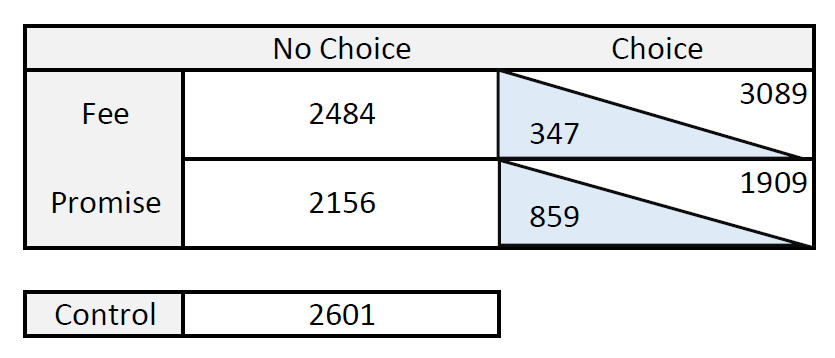
\includegraphics[width=0.70\textwidth]{Figuras/exp_arms.PNG}
    \end{center}
\end{frame}


\begin{frame}{Branches and Timeline}
    \begin{itemize}
        \item We worked on 6 branches during 2012
        \item We observe transactions for about 30 days before and 6 months after the experiment ends.
    \end{itemize}
    \begin{center}
        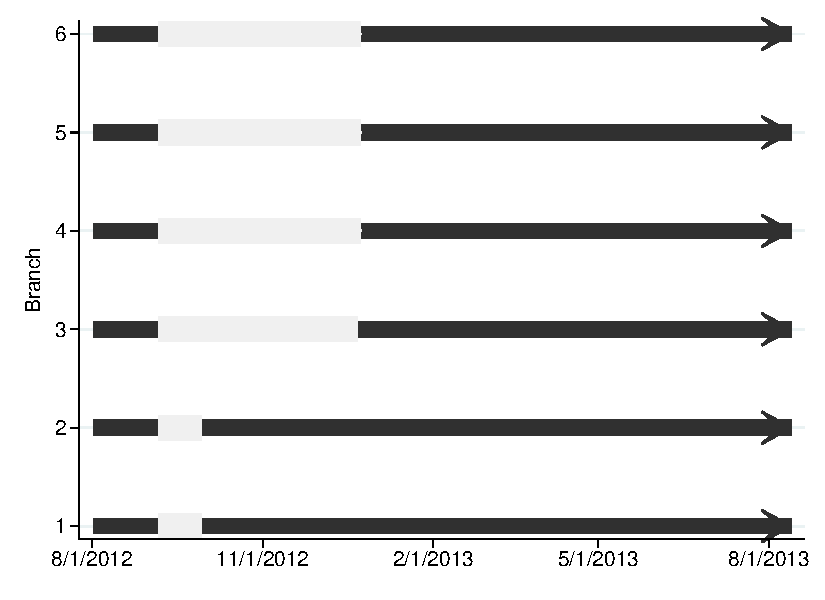
\includegraphics[width=0.80\textwidth]{Figuras/timeline_suc_exp_extended.pdf}
    \end{center}
\end{frame}


\begin{frame}{Data}

\begin{itemize}
    \item Admin data:
    \begin{itemize}
        \item Date of pawning
        \item Value of item --> loan size
        \item Dates of payments and amounts, 
        \item Whether borrower recovered item
        \item Borrower id
    \end{itemize}
    \vfill
    \item Survey data: Own 2 page questionnaire at the branch before pawning
    \begin{itemize}
        \item Some demographics
        \item Vulnerability
        \item Cost of going to branch
        \item 3 ``self control'' questions
        \item ... others.
    \end{itemize}
\end{itemize}
    
\end{frame}


\begin{frame}{Survey questions}
    \begin{enumerate}
        \item Family
            \begin{itemize}
                \item Common asks - Is it common family or friends ask you for money?
            \end{itemize}
        \item Income 
        \begin{itemize}
            \item In the last six months, did you need money to pay...?
        \end{itemize}
        \item Self-Control
        \begin{itemize}
            \item Makes budget - Do you budget your monthly expenses?
            \item Present bias - Prefers 100 tomorrow over 250 in a month AND 150 in 4 months over 100 in 3 months
            \item Reminder - Would you like to receive free reminders on your cell phone?
            \item Tempt - Has it happened to you that you spend more than you would like because you fall into temptation?
        \end{itemize}
        \item Experience
        \begin{itemize}
            \item Rosca - Do you participate in a \textit{rosca} or in a savings account?
            \item Pawn before - Have you pawn before?
        \end{itemize}
        \item Other
            \begin{itemize}
            \item Low time - Below median in reported time to arrive to the pawn shop.
            \item Low cost - Below median in reported cost spent to arrive to the pawn shop
            \item Prob recovery - From 0 to 100 mark with an X how sure you are to recover your garment
            \item Stressed - How often do you feel stressed by your household economic situation? - 0 when answered `never' and 1 otherwise
        \end{itemize}
    \end{enumerate}
\end{frame}


\begin{frame}{SS Histograms}

\begin{figure}[H]
    \label{nochoicehte_takeup_pred}
    \begin{center}
     \begin{subfigure}{0.45\textwidth}
        \caption{In the last six months, did you need money to pay...?}
        \centering
        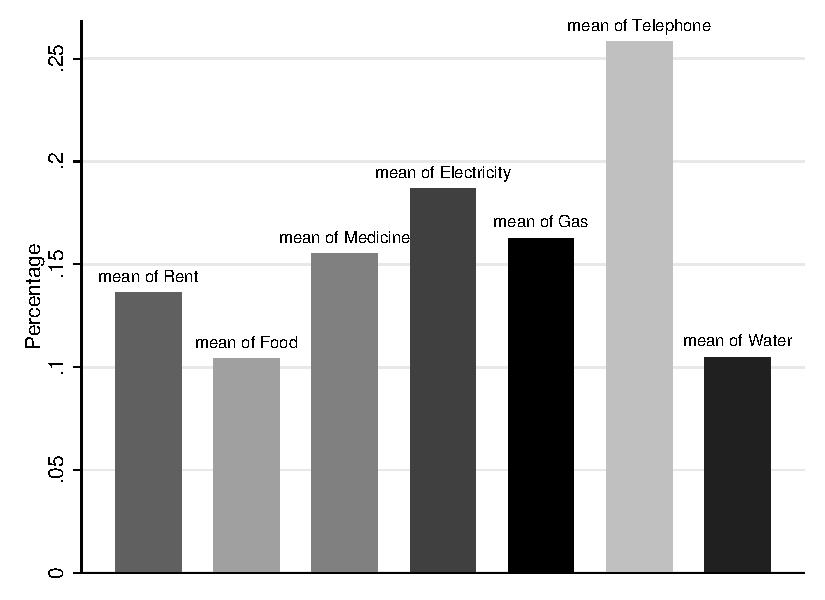
\includegraphics[width=\textwidth]{Figuras/perc_utilities.pdf}
    \end{subfigure}
     \begin{subfigure}{0.45\textwidth}
        \caption{Cost and Time to arrive to pawn shop}
        \centering
        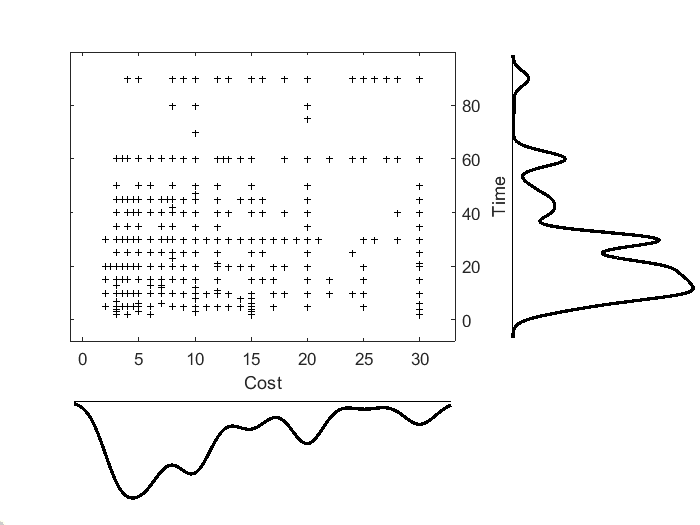
\includegraphics[width=\textwidth]{Figuras/cost_time_scatter_hist.png}
    \end{subfigure}
    \end{center}
    \end{figure}
    
\end{frame}



\begin{frame}{Summary Stats}
    \begin{table}
        \begin{center}
        \tiny{% Table generated by Excel2LaTeX from sheet 'SS'
\begin{tabular}{lcccccccc}
\toprule
      &       &       & \multicolumn{5}{c}{Treatment arms}    &  \\
\midrule
      &       &       &       & \multicolumn{2}{c}{No Choice } & \multicolumn{2}{c}{Choice} &  \\
\midrule
\midrule
      & Overall & Pre-experiment & Control & Fee   & Promise & Fee   & Promise & p-value \\
\midrule
      & \multicolumn{8}{c}{Panel A : Administrative Data} \\
\midrule
\midrule
Loan amount  & 2197  & 2239  & 2301  & 2147  & 2133  & 2181  & 2089  & 0.32 \\
      & (25)  & (39)  & (79)  & (72)  & (74)  & (65)  & (65)  &  \\
Monday & 0.18  & 0.16  & 0.18  & 0.16  & 0.17  & 0.19  & 0.21  & 0.96 \\
      & (0.02) & (0.03) & (0.05) & (0.05) & (0.06) & (0.06) & (0.05) &  \\
Number of branch-day pawns & 34    & 36    & 31    & 31    & 32    & 37    & 34    & 0.38 \\
      & (0.82) & (1.25) & (2.2) & (2.35) & (2.38) & (2.65) & (1.76) &  \\
\midrule
Number of branch-days & -     &       & 84    & 80    & 68    & 93    & 82    &  \\
Obs   & 21808 & 8366  & 2601  & 2484  & 2156  & 3435  & 2766  &  \\
\midrule
      & \multicolumn{8}{c}{Panel B : Survey Data (conditional on pawning)} \\
\midrule
\midrule
Woman & 0.73  &       & 0.76  & 0.72  & 0.73  & 0.72  & 0.74  & 0.41 \\
      & (0.01) &       & (0.02) & (0.02) & (0.02) & (0.02) & (0.01) &  \\
Age   & 43.31 &       & 43.16 & 43.17 & 42.96 & 43.96 & 43.06 & 0.79 \\
      & (0.28) &       & (0.57) & (0.79) & (0.65) & (0.61) & (0.52) &  \\
Subjective value & 3068  &       & 3151  & 2978  & 2985  & 3114  & 3079  & 0.41 \\
      & (39)  &       & (69)  & (91)  & (76)  & (85)  & (100) &  \\
Has pawn before & 0.9   &       & 0.89  & 0.9   & 0.89  & 0.91  & 0.89  & 0.68 \\
      & (0)   &       & (0.01) & (0.01) & (0.01) & (0.01) & (0.01) &  \\
Subj. pr. of recovery & 93.14 &       & 92.74 & 92.16 & 93.6  & 93.67 & 93.3  & 0.46 \\
      & (0)   &       & (0.55) & (0.86) & (0.6) & (0.47) & (0.6) &  \\
+High-school & 0.66  &       & 0.66  & 0.67  & 0.65  & 0.67  & 0.64  & 0.74 \\
      & (0.01) &       & (0.02) & (0.02) & (0.02) & (0.02) & (0.02) &  \\
Survey response rate & 0.78  &       & 0.77  & 0.75  & 0.8   & 0.77  & 0.79  & 0.5 \\
      & (0.01) &       & (0.02) & (0.03) & (0.02) & (0.02) & (0.02) &  \\
\midrule
Obs   & 10431 &       & 2000  & 1855  & 1732  & 2652  & 2192  &  \\
\midrule
\midrule
      & \multicolumn{8}{c}{Panel C : Survey Data (unconditional)} \\
\midrule
\midrule
Woman & 0.74  & 0.75  & 0.76  & 0.72  & 0.73  & 0.72  & 0.74  & 0.32 \\
      & (0.01) & (0.01) & (0.02) & (0.02) & (0.02) & (0.02) & (0.01) &  \\
Age   & 43.24 & 43.06 & 43.2  & 43.21 & 43.01 & 44.07 & 43.07 & 0.79 \\
      & (0.21) & (0.32) & (0.56) & (0.77) & (0.66) & (0.61) & (0.51) &  \\
Subjective value & 3112  & 3192  & 3145  & 2985  & 3010  & 3111  & 3082  & 0.41 \\
      & (36)  & (75)  & (68)  & (88)  & (76)  & (84)  & (99)  &  \\
Has pawn before & 0.89  & 0.88  & 0.89  & 0.9   & 0.89  & 0.91  & 0.89  & 0.56 \\
      & (0.01) & (0.01) & (0.01) & (0.01) & (0.01) & (0.01) & (0.01) &  \\
Subj. pr. of recovery & 92.64 & 91.84 & 92.73 & 92.19 & 93.66 & 93.71 & 93.34 & 0 \\
      & (0.2) & (0.31) & (0.54) & (0.84) & (0.59) & (0.46) & (0.59) &  \\
+High-school & 0.63  & 0.6   & 0.66  & 0.67  & 0.65  & 0.66  & 0.64  & 0.01 \\
      & (0.01) & (0.01) & (0.02) & (0.02) & (0.02) & (0.02) & (0.02) &  \\
\% ended up pawning &       &       & 0.98  & 0.97  & 0.99  & 0.98  & 0.99  & 0.25 \\
\midrule
Obs   & 17546 & 6919  & 2035  & 1907  & 1757  & 2710  & 2218  &  \\
\bottomrule
\bottomrule
\end{tabular}%
}
        \end{center}
    \end{table}
\end{frame}




\section{Results on Payments and Recovery}

\begin{frame}{When do borrowers pay?}
    \begin{center}
        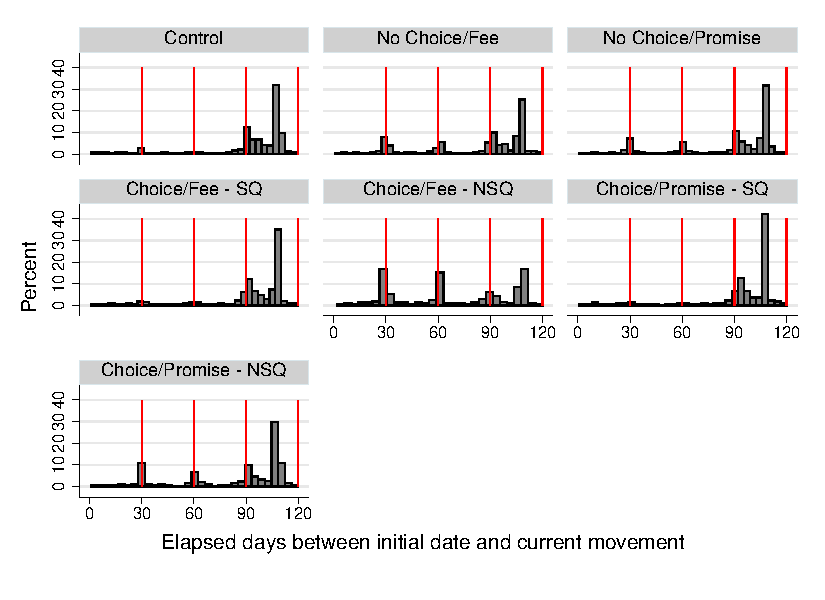
\includegraphics[width=\textwidth]{Figuras/hist_payments.pdf}
    \end{center}
\end{frame}


\begin{frame}{Recovering Piece}

    \begin{center}
        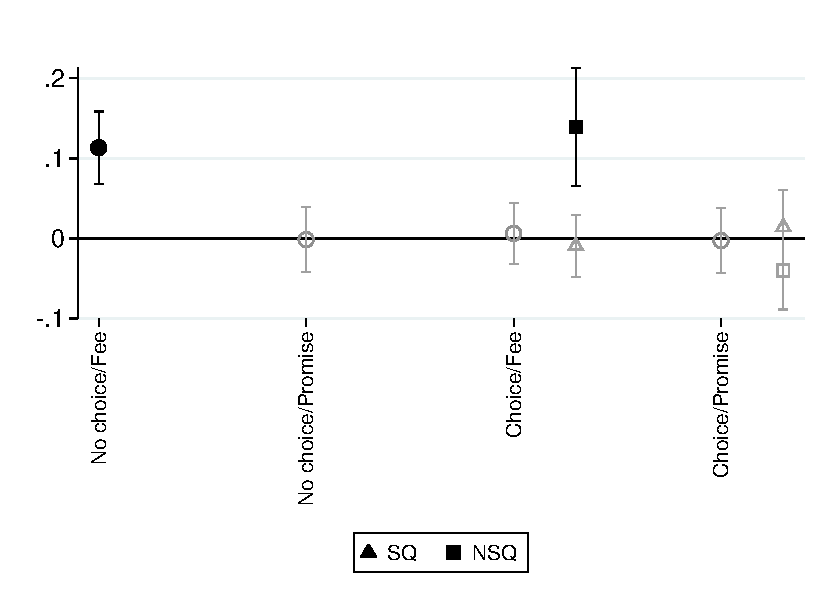
\includegraphics[width=.70\textwidth]{Figuras/te_graph_des_c.pdf}
    \end{center}
\end{frame}


\begin{frame}{Number of Payments}
    \begin{center}
        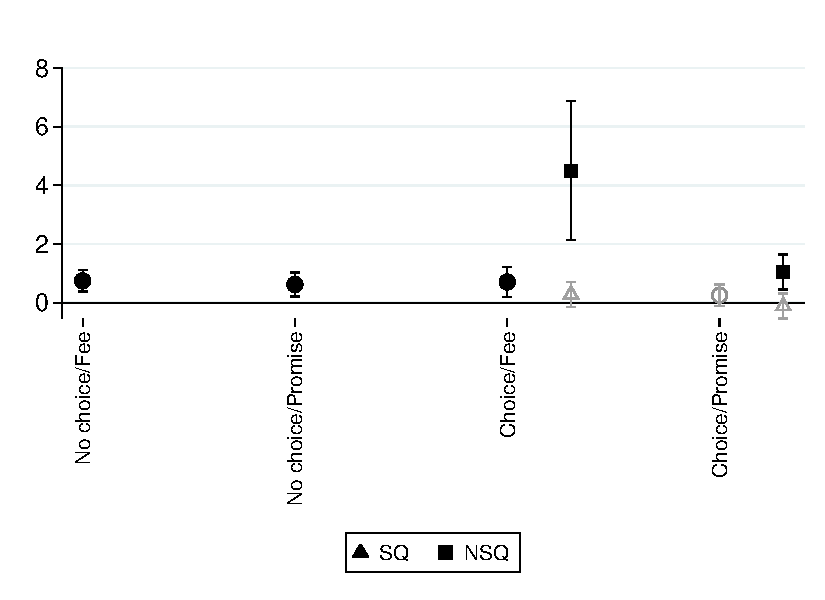
\includegraphics[width=.70\textwidth]{Figuras/te_graph_num_p.pdf}
    \end{center}
\end{frame}


\begin{frame}{Percentage of Loan paid}
    \begin{center}
        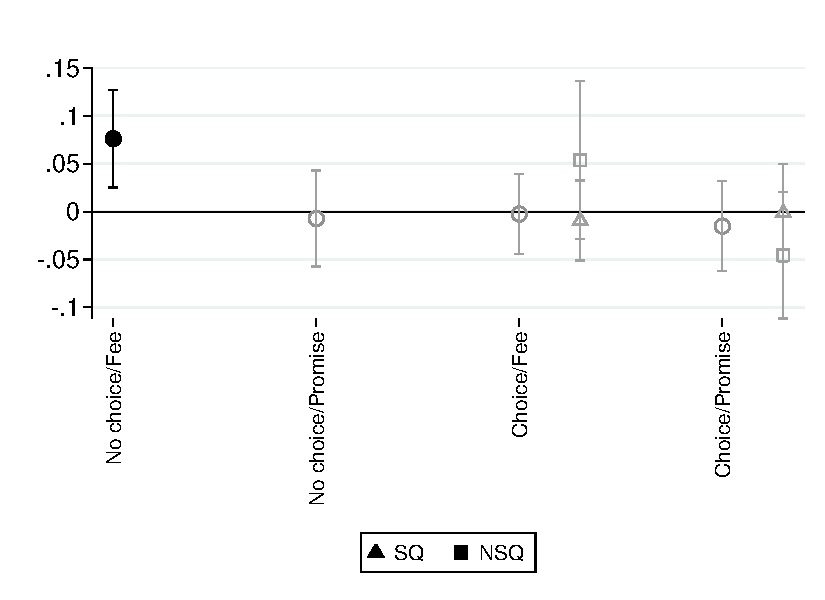
\includegraphics[width=.70\textwidth]{Figuras/te_graph_sum_porcp_c.pdf}
    \end{center}
\end{frame}


\begin{frame}{Days to recover piece | recovering}
    \begin{center}
        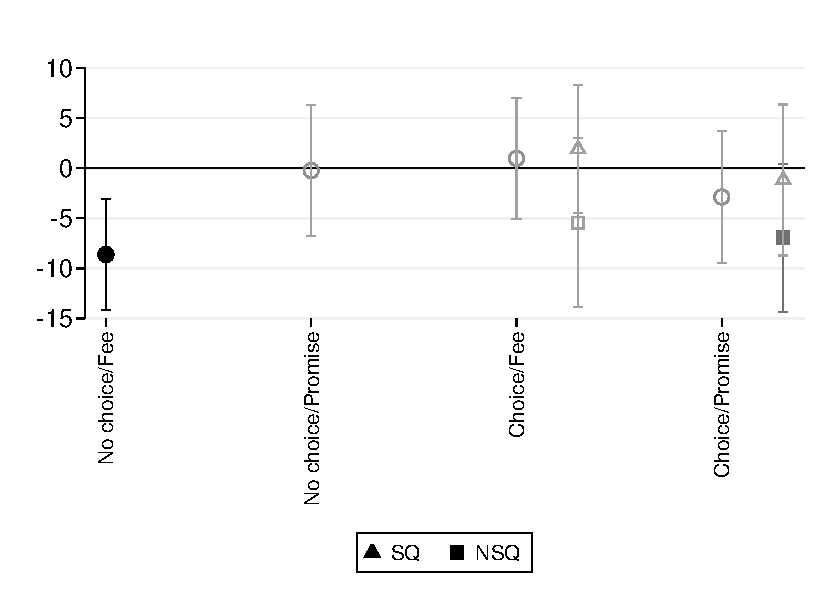
\includegraphics[width=.70\textwidth]{Figuras/te_graph_dias_al_desempenyo.pdf}
    \end{center}
\end{frame}


\begin{frame}{Reincidence}
    \begin{center}
        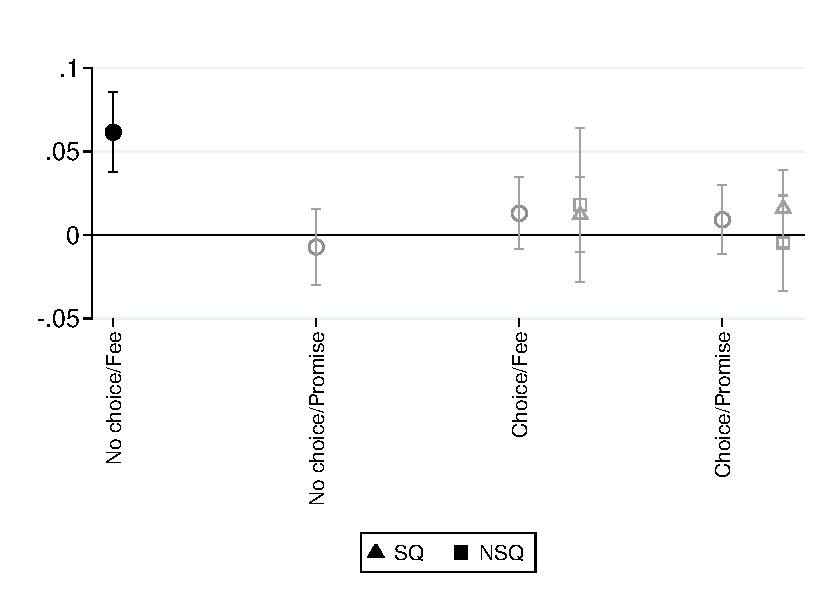
\includegraphics[width=.70\textwidth]{Figuras/te_graph_reincidence.pdf}
    \end{center}
\end{frame}



\begin{frame}[label = hte]{TE heterogeneity in Recovering}
    \begin{center}
        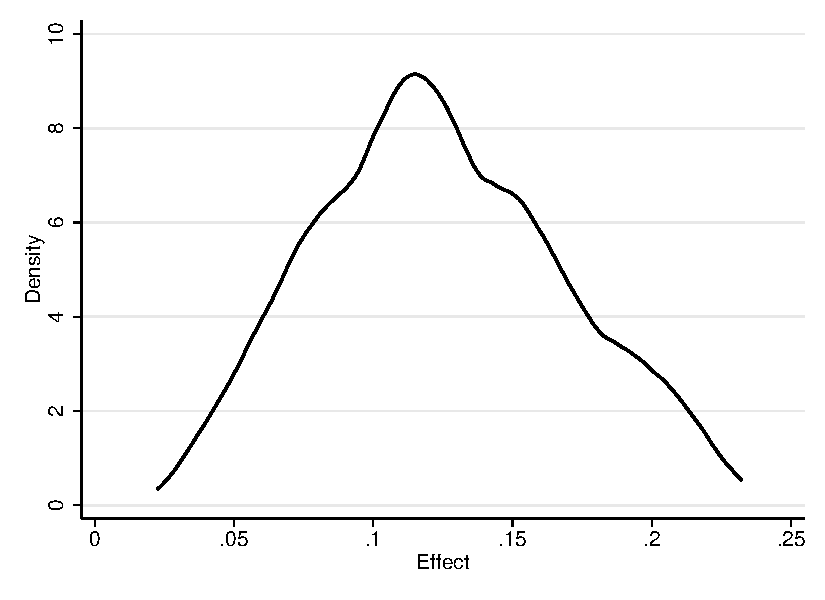
\includegraphics[width=.80\textwidth]{Figuras/he_dist_des_c_pro_2.pdf}
    \end{center}
    
 Based on \hyperlink{GRF}{\beamerbutton{GRF}}   
\end{frame}


\begin{frame}{Some determinants of TE - The nature of heterogeneity}
    \begin{center}
        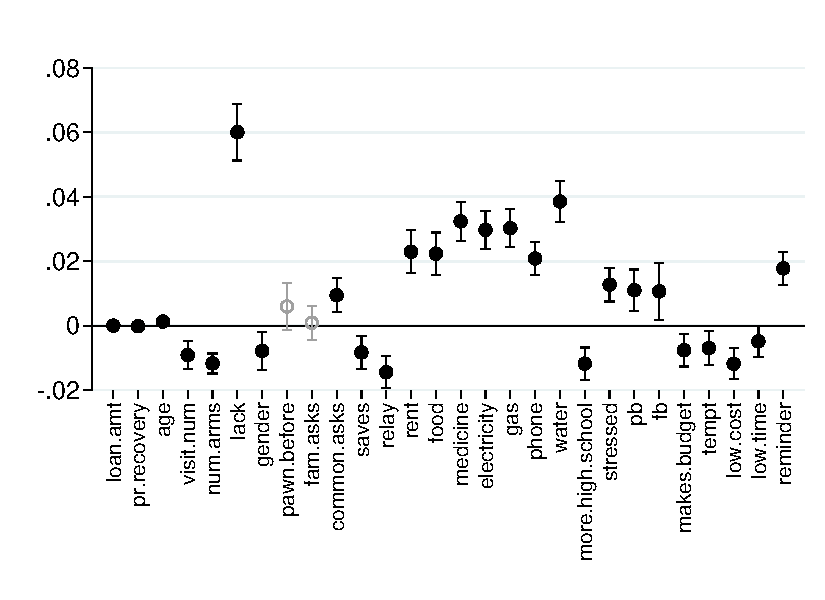
\includegraphics[width=.9\textwidth]{Figuras/HE/he_int_des_c_pro_2.pdf}
    \end{center}
\end{frame}




\section{Results on Demand for Commitment}

\begin{frame}{10\% take up with fee: who are they?}
    \begin{center}
        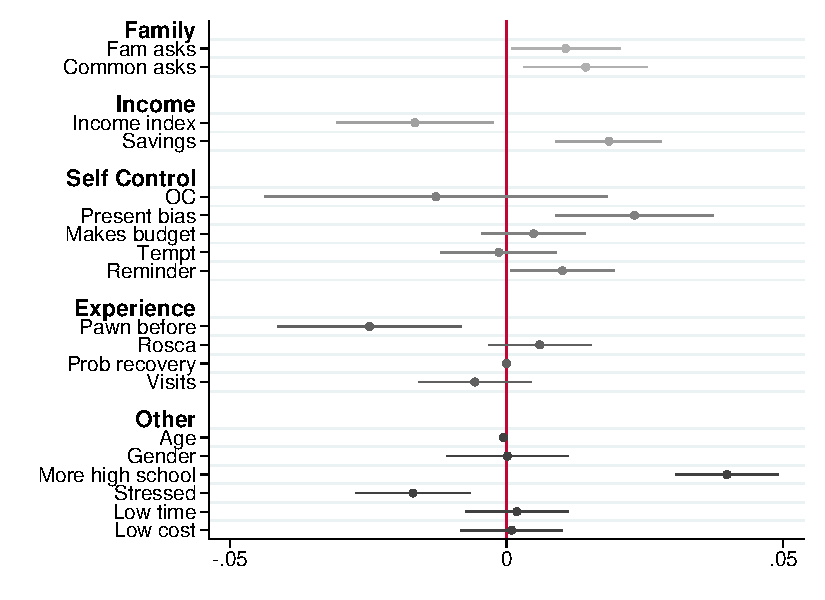
\includegraphics[width=.90\textwidth]{Figuras/pago_frec_vol_fee_interactions_rf.pdf}
    \end{center}
\end{frame}



\begin{frame}{Those taking up are not those with highest TE}
    \begin{center}
        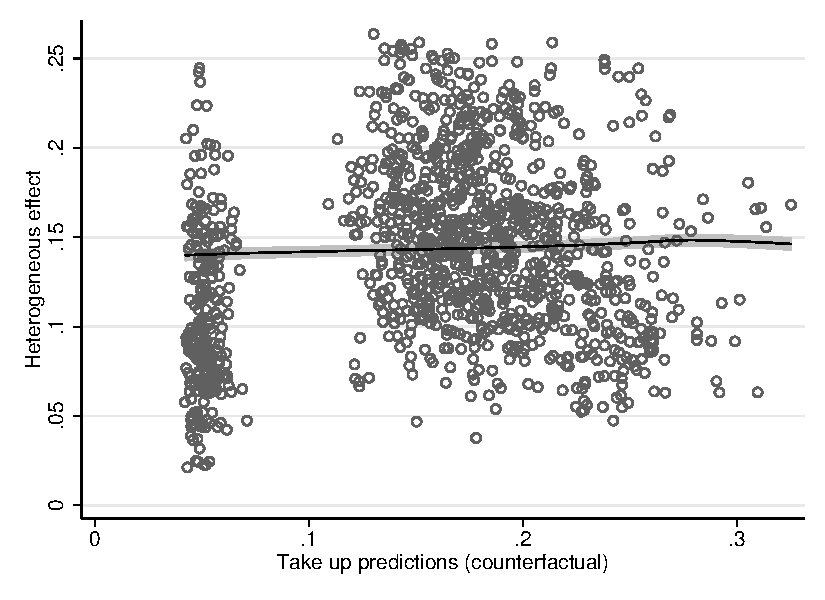
\includegraphics[width=.70\textwidth]{Figuras/takeup_he_pro_2_fee.pdf}
    \end{center}
\end{frame}



\section{Next steps}

\begin{frame}{Next steps}

\begin{itemize}
    \item Can a simple neoclassical model explain quantitatively the results?
    \vfill
    \item Estimate a model and talk about welfare?
    \vfill
    \item What about naive present-biased consumers? Can we separate them?
    \vfill
    \item Does promise commitment work for some people?
    \vfill
    \item Does frequent payment cause lack of payment of basic services or other loans?
\end{itemize}
    
\end{frame}



\section{Appendix}

\begin{frame}{Explanation in ``choice'' days}
    \begin{center}
        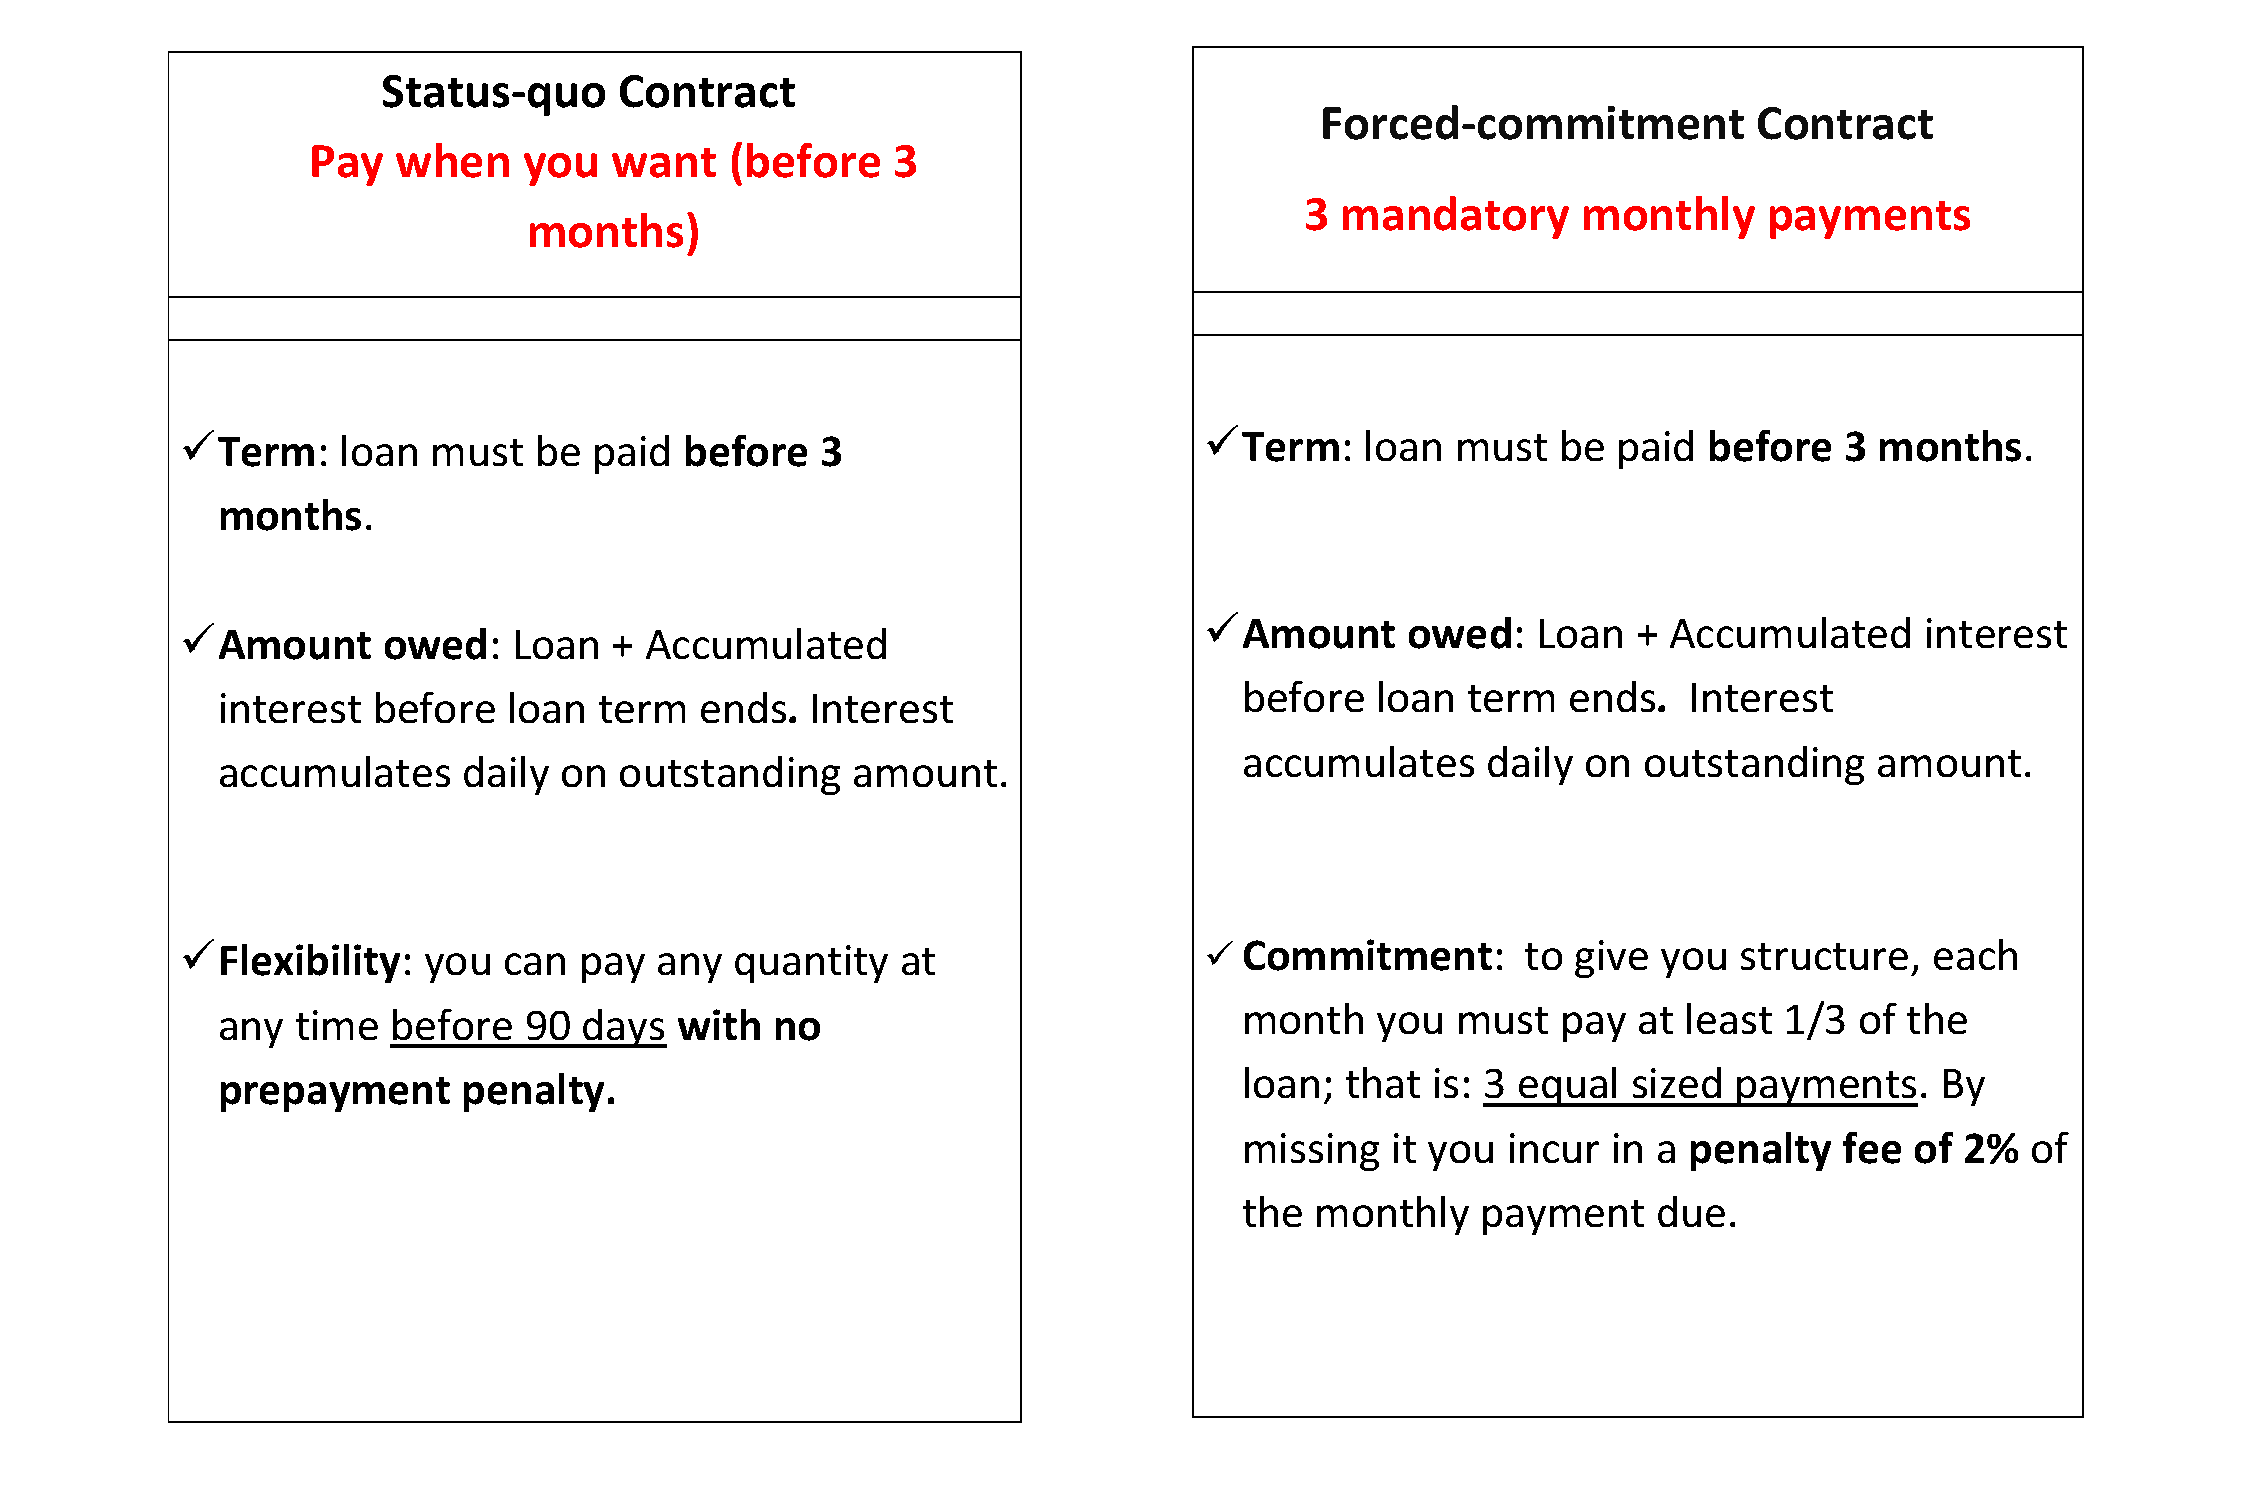
\includegraphics[width=\textwidth]{Figuras/micas.pdf}
    \end{center}
\end{frame}


\begin{frame}{Histograms Percentage Paid}
    \begin{center}
        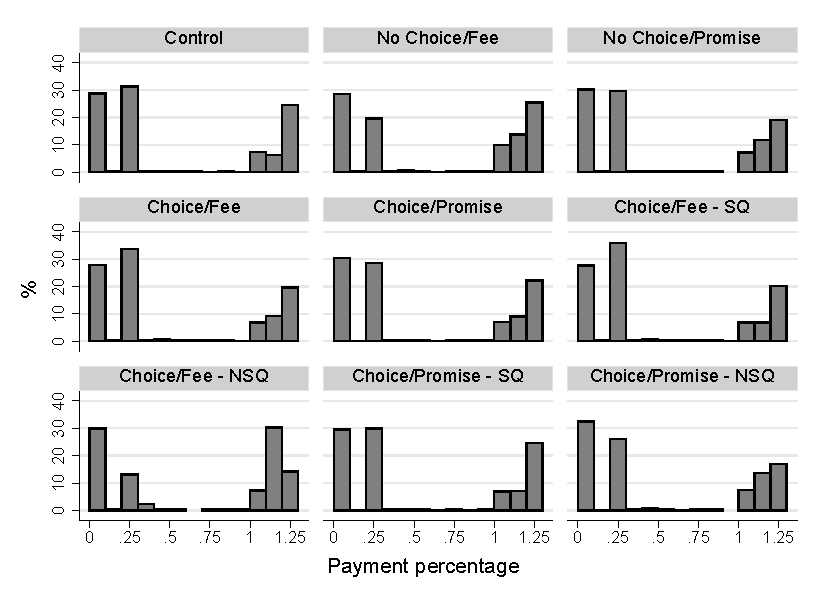
\includegraphics[width=.9\textwidth]{Figuras/hist_perc_payment.pdf}
    \end{center}
\end{frame}



\begin{frame}{Characteristics of present bias}
\begin{table}[H]
\label{pb_chars}
\begin{center}
\tiny{% Table generated by Excel2LaTeX from sheet 'pb_chars'
\begin{tabular}{lcccccc}
\toprule
\multicolumn{1}{|r}{} & \multicolumn{3}{c}{Present bias} & \multicolumn{3}{c|}{Future bias} \\
\midrule
      & Pooled & Female & Male  & Pooled & Female & Male \\
\midrule
\midrule
      & (1)   & (2)   & (3)   & (4)   & (5)   & (6) \\
\midrule
\midrule
Woman & 0.016 &       &       & -0.0068 &       &  \\
      & (0.014) &       &       & (0.011) &       &  \\
Age   & -0.00019 & -0.00025 & 0.00022 & 0.00090** & 0.00077* & 0.0012* \\
      & (0.00048) & (0.00058) & (0.00084) & (0.00036) & (0.00043) & (0.00067) \\
Needs money to pay utilities & -0.024 & -0.014 & -0.058 & -0.023 & -0.020 & -0.035 \\
      & (0.022) & (0.026) & (0.041) & (0.015) & (0.018) & (0.027) \\
Family asks for money & -0.00054 & -0.016 & 0.042 & -0.0091 & -0.0098 & -0.0055 \\
      & (0.013) & (0.016) & (0.026) & (0.010) & (0.012) & (0.020) \\
Tempted & 0.018 & 0.025 & -0.0071 & 0.018* & 0.023** & 0.0029 \\
      & (0.013) & (0.015) & (0.027) & (0.0098) & (0.011) & (0.021) \\
Reminder & 0.035** & 0.041** & 0.019 & 0.023** & 0.016 & 0.042* \\
      & (0.014) & (0.017) & (0.025) & (0.011) & (0.012) & (0.021) \\
Subjective prob & -0.00098** & -0.00091* & -0.0013 & 0.00011 & -0.00013 & 0.00085** \\
      & (0.00042) & (0.00048) & (0.00092) & (0.00027) & (0.00033) & (0.00038) \\
Makes budget & 0.00041 & 0.0038 & -0.0075 & -0.016* & -0.013 & -0.022 \\
      & (0.013) & (0.015) & (0.024) & (0.0097) & (0.011) & (0.019) \\
Pawn before & -0.034 & -0.020 & -0.059 & -0.026* & -0.0086 & -0.059* \\
      & (0.021) & (0.026) & (0.036) & (0.016) & (0.018) & (0.031) \\
Rosca & 0.032** & 0.023 & 0.057** & 0.022** & 0.014 & 0.043** \\
      & (0.013) & (0.015) & (0.025) & (0.0098) & (0.011) & (0.020) \\
Constant  & 0.24*** & 0.24*** & 0.28*** & 0.048 & 0.053 & -0.0040 \\
      & (0.051) & (0.057) & (0.11) & (0.031) & (0.037) & (0.050) \\
\midrule
      &       &       &       &       &       &  \\
Observations & 3510  & 2565  & 945   & 3510  & 2565  & 945 \\
R-sq  & 0.008 & 0.007 & 0.018 & 0.007 & 0.005 & 0.023 \\
\bottomrule
\bottomrule
\end{tabular}%
}
\end{center}
\end{table}
\end{frame}



\begin{frame}{30\% take up with promise: Different relation with self control}
    \begin{center}
        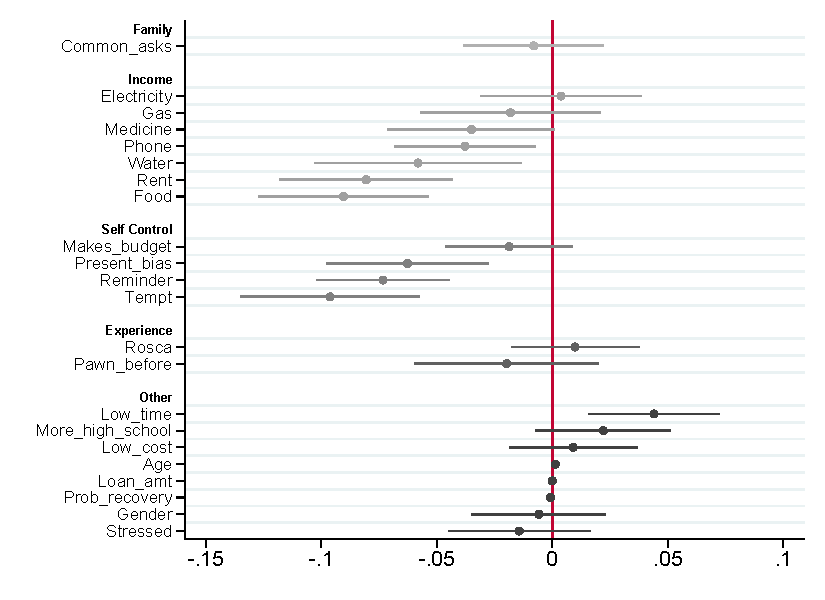
\includegraphics[width=.90\textwidth]{Figuras/pago_frec_vol_promise_interactions_rf.pdf}
    \end{center}
\end{frame}


\begin{frame}{ML fit}
    \begin{center}
    \scriptsize
    % Table generated by Excel2LaTeX from sheet 'oos_pago_frec_vol_fee'
\begin{tabular}{lcccc}
\toprule
      & \multicolumn{4}{c}{Frequent voluntary payment - FEE} \\
\midrule
\midrule
OOS measures & Logit & SW-Logit & RF    & Boosting \\
\midrule
\midrule
MAE   & 0.21  & 0.21  & 0.23  & 0.17 \\
MSE   & 0.1   & 0.1   & 0.1   & 0.09 \\
AUC (out of sample) & 0.76  & 0.78  & 0.84  & 0.85 \\
      & (0.06) & (0.06) & (0.06) & (0.05) \\
AUC (in sample) & 0.84  & 0.82  & 0.92  & 0.99 \\
      & (0.02) & (0.02) & (0.01) & (0.01) \\
Accuracy & 0.82  & 0.84  & 0.86  & 0.88 \\
Correlation (0-1) & 0.13  & 0.26  & 0.37  & 0.31 \\
Correlation (predicted val) & 0.33  & 0.38  & 0.37  & 0.43 \\
R-squared  & 0.08  & 0.13  & 0.11  & 0.19 \\
Expected value of predictions & 0.17  & 0.17  & 0.16  & 0.12 \\
\bottomrule
\bottomrule
\end{tabular}%

    \end{center}
\end{frame}




\begin{frame}{Exit survey}
    \begin{center}
    \tiny
    % Table generated by Excel2LaTeX from sheet 'SS'
\begin{tabular}{lccccccc}
\toprule
\multicolumn{8}{c}{Exit Survey Data} \\
\midrule
\midrule
      &       &       & \multicolumn{2}{c}{No Choice } & \multicolumn{2}{c}{Choice} &  \\
\midrule
\midrule
      & Overall & Control & Fee   & Promise & Fee   & Promise & p-value \\
\midrule
      & \multicolumn{7}{c}{Panel A: Outcomes} \\
\midrule
\midrule
Will reincide & 0.94  & 0.96  & 0.95  & 0.96  & 0.94  & 0.92  & 0.6 \\
      & (0.01) & (0.01) & (0.02) & (0.02) & (0.02) & (0.03) &  \\
Very satisfied & 0.34  & 0.36  & 0.32  & 0.33  & 0.33  & 0.36  & 0.95 \\
      & (0.02) & (0.05) & (0.05) & (0.05) & (0.04) & (0.04) &  \\
Better econ situation & 0.42  & 0.53  & 0.29*** & 0.35** & 0.44  & 0.47  & 0.02 \\
      & (0.03) & (0.06) & (0.05) & (0.06) & (0.05) & (0.04) &  \\
Choose frequent payment & 0.63  & 0.65  & 0.58  & 0.58  & 0.58  & 0.77** & 0 \\
      & (0.02) & (0.05) & (0.05) & (0.06) & (0.04) & (0.03) &  \\
\midrule
      & \multicolumn{7}{c}{Panel B: Balance} \\
\midrule
\midrule
Loan amount  & 1957.72 & 1940.41 & 1926  & 2006.83 & 2002.97 & 1892.54 & 0.98 \\
      & (67.84) & (160.03) & (150.89) & (187.56) & (114.96) & (157.83) &  \\
Woman & 0.71  & 0.69  & 0.72  & 0.77  & 0.66  & 0.73  & 0.58 \\
      & (0.02) & (0.05) & (0.06) & (0.05) & (0.05) & (0.04) &  \\
Age   & 43.98 & 42.84 & 46.27 & 43.82 & 44.57 & 42.24 & 0.29 \\
      & (0.59) & (1.33) & (1.74) & (1.1) & (0.99) & (1.16) &  \\
Subjective value & 3166.31 & 3448.99 & 3182.11 & 3049.88 & 3074.69 & 3081.52 & 0.85 \\
      & (120.82) & (288.38) & (286.2) & (303.87) & (210.79) & (296.63) &  \\
Has pawn before & 0.88  & 0.84  & 0.9   & 0.87  & 0.95** & 0.8   & 0.01 \\
      & (0.02) & (0.05) & (0.03) & (0.05) & (0.02) & (0.05) &  \\
Subj. pr. of recovery & 95.35 & 94.5  & 94.84 & 96.6  & 95.06 & 95.87 & 0.82 \\
      & (0.56) & (1.4) & (1.21) & (1.5) & (1.01) & (1.09) &  \\
+High-school & 0.66  & 0.72  & 0.63  & 0.65  & 0.67  & 0.64  & 0.84 \\
      & (0.03) & (0.06) & (0.06) & (0.07) & (0.05) & (0.06) &  \\
\midrule
Obs   & 905   & 175   & 154   & 172   & 234   & 170   &  \\
\bottomrule
\bottomrule
\end{tabular}%

    \end{center}
\end{frame}



\begin{frame}[label = GRF]{Generalized Random Forests}

A method for non-parametric statistical estimation based on RF
for estimating $\theta(x)$ that can be identified as the solution to a set of local moment equations:

\[\mathbb{E}[\psi(Z,\theta,h(x,W))\;|\;X=x]=0\]

where $\psi$ is a known score function and $h$ is an unknown nuisance function also estimated from data.\\

\vspace{5mm}

The main application involves HTE. To achieve this, the method seeks trees that, when combined, produces leaves that maximizes heterogeneity. In other words, it splits the data that produce the biggest difference in TE across leaves, by still producing accurate estimates of the TE. Moreover, the splits are made honest by taking the training data and splitting it into two subsamples: a splitting subsample and an estimating subsample. The estimates being calculated on the latter. \hyperlink{hte}{\beamerbutton{Back}}\\

\end{frame}



\begin{frame}{Honest Causal Tree construction}
Given a dataset with an outcome $Y$, covariates $X$, and a randomized condition $W$ that takes on the value of 0 for control and 1 for treatment:

\begin{enumerate}
\item Split the data into subsample $I$ and subsample $J$

\item Train a decision tree on subsample $I$ predicting $Y$ from $X$, with the requirement that each terminal node has at least $k$ observations from each condition in subsample $J$

\item Apply the decision tree constructed on subsample $I$ to subsample $J$

\item At each terminal node, get the mean of predictions for the $W = 1$ cases from subsample $J$ and subtract the mean of predictions for the $W = 0$ cases from subsample $J$; the resulting difference is the estimated treatment effect.

\end{enumerate}

This is then applied to a causal random forest by using bagging or bootstrapping

\end{frame}
\end{document}

